\documentclass{report}


\input{preamble}
\input{macros}
\input{letterfonts}

\title{\Huge{Teoria dos Grafos e Computabilidade}\\Resumos}
\author{\huge{Pedro Marçal Lima}}
\date{}

\begin{document}

\maketitle
\newpage% or \cleardoublepage
% \pdfbookmark[<level>]{<title>}{<dest>}
\pdfbookmark[section]{\contentsname}{toc}
\tableofcontents
\pagebreak
\chapter{Introdução}
\section{O Que é um Grafo?}

\dfnc{Grafo}{
	Um grafo é um conjunto de pontos (vértices) e suas relações (arestas):
	\[
		G = (V, E)
	\]
	onde:
	\[
		V = \{v_1, v_2, \dots, v_n\}, \quad E = \{\{v_1, v_2\}, \{v_2, v_3\}, \dots\}
	\]
}
\section{Grafo não-direcionado}
Um grafo não-direcionado, se trata de um grafo
\[
	G = (V, E)
\]
em que suas arestas $(v_i, v_j)$ e $(v_j, v_i)$ são idênticas, ou seja, não importa a direção da aresta, qualquer aresta pode ser tanto de "ida" quanto de "volta".

\begin{center}
	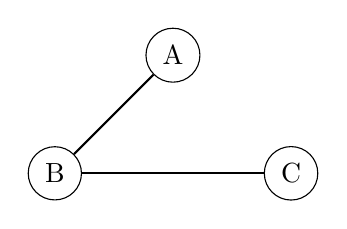
\begin{tikzpicture}[scale=1.5]

		\node[draw,circle] (A) at (0, 1) {A};
		\node[draw,circle] (B) at (-1, 0) {B};
		\node[draw,circle] (C) at (1, 0) {C};

		\foreach \source/\dest in {A/B,  B/C}
		\draw[thick] (\source) -- (\dest);

	\end{tikzpicture}
\end{center}

\dfn{Grafo Não Direcionado}{
	\[
		G = (V, E)
	\]
	onde:
	\[
		\begin{aligned}
			V & = \{v_1, v_2, \dots, v_n\}             \\
			E & = \{\{v_i, v_j\} \mid v_i, v_j \in V\} \\
			E & \subseteq V \times V
		\end{aligned}
	\]
	\[
		\{v_i, v_j\} = \{v_j, v_i\}
	\]
}
\section{Grafo direcionado}
Um grafo direcionado, se trata de um grafo
\[
	G = (V, E)
\]
em que suas arestas $(v_i, v_j)$ e $(v_j, v_i)$ são diferentes, ou seja, a direção da aresta é relevante, sendo assim, considerada uma aresta de saída ou entrada em relação a um vértice.

\begin{center}
	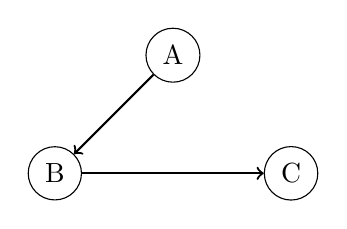
\begin{tikzpicture}[scale=1.5]

		\node[draw,circle] (A) at (0, 1) {A};
		\node[draw,circle] (B) at (-1, 0) {B};
		\node[draw,circle] (C) at (1, 0) {C};

		\foreach \source/\dest in {A/B, B/C}
		\draw[->,thick] (\source) -- (\dest);

	\end{tikzpicture}
\end{center}

\dfn{Grafo Direcionado}{
	\[
		G = (V, E)
	\]
	onde:
	\[
		\begin{aligned}
			V & = \{v_1, v_2, \dots, v_n\}           \\
			E & = \{(v_i, v_j) \mid v_i, v_j \in V\} \\
			E & \subseteq V \times V
		\end{aligned}
	\]
	\[
		(v_i, v_j) \neq (v_j, v_i)
	\]
}
\nt{Importante notar que, na representação de arestas, utiliza-se de $\{ \}$ para represenar um par não ordenado(a ordem não importa), e $( )$ para representar um par ordenado(a ordem importa)}

\section{Conceitos de vértices}
\subsection{Vértices adjacentes(vizinhos)}
Vértices podem ser considerandos adjacentes ou vizinhos caso possuam uma aresta de ligação entre eles

\begin{center}
	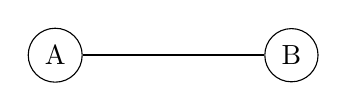
\begin{tikzpicture}[scale=1.5]

		\node[draw,circle] (A) at (0, 0) {A};
		\node[draw,circle] (B) at (2, 0) {B};

		\draw[-,thick] (A) to (B);

	\end{tikzpicture}
\end{center}
\dfnc{Vértices adjacentes}{
	Dado dois vértices:
	\[
		v_i \text{ e } v_j
	\]
	onde:
	\[
		v_i \land v_j \in V
	\]
	\[
		(v_i, v_j) \in E
	\]
	Entende-se que:
	\[
		v_i \leftrightarrow v_j
	\]
}

\subsection{Vértice isolado}
É um vértice v que possui $d(v)= 0$, ou seu conjunto de arestas vazio(como D e C no grafo abaixo).
\begin{center}
	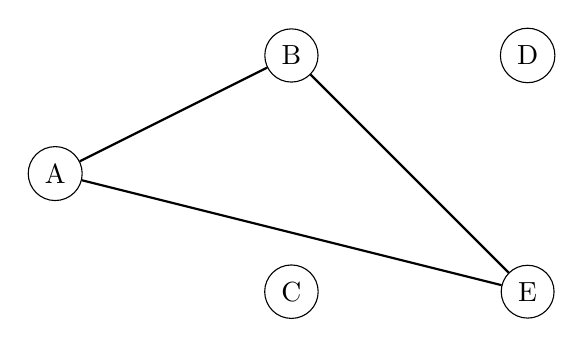
\begin{tikzpicture}[scale=1.5]

		\node[draw,circle] (A) at (0, 0) {A};
		\node[draw,circle] (B) at (2, 1) {B};
		\node[draw,circle] (C) at (2, -1) {C};
		\node[draw,circle] (D) at (4, 1) {D};
		\node[draw,circle] (E) at (4, -1) {E};

		\draw[thick] (A) -- (B);

		\draw[thick] (A) -- (E);

		\draw[thick] (E) to (B);


	\end{tikzpicture}

\end{center}

\dfnc{Vértice Isolado}{
	Dado um grafo
	\[
		G = (V, E)
	\]
	onde:
	\[
		v \in V
	\]
	temos que:
	\[
		\begin{cases}
			\forall\, u \in V, \quad \{v, u\} \notin E                     & \text{(se } G \text{ é não direcionado)} \\
			\forall\, u \in V, \quad (u, v) \notin E \land (v, u) \notin E & \text{(se } G \text{ é direcionado)}
		\end{cases}
	\]
	ou:
	\[
		\begin{cases}
			d(v) = 0            & \text{(se } G \text{ é não direcionado)} \\
			d^+(v) + d^-(v) = 0 & \text{(se } G \text{ é direcionado)}     \\
		\end{cases}
	\]
	Portanto, podemos concluir que \( v \) é um vértice isolado, pois:
	\[
		N(v) = \emptyset
	\]

}

\nt{A expressão $N(v)$ se refere ao conjunto vizinhança de um vértice (neighborhood), ou seja, os vértices que ele possui ligação por uma aresta}

\section{Aresta incidente}
Caso um vértice v, seja o vértice final de uma aresta $e = {u,v}$, $e$ é incidente em $v$ a partir de $u$

\dfnc{Aresta incidente}{
	Em um grafo G = (V, E), uma aresta incidente $e$ em $v$, é uma aresta $e$ = $(u,v)$


}

\begin{center}
	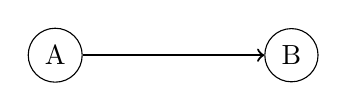
\begin{tikzpicture}[scale=1.5]

		\node[draw,circle] (A) at (0, 0) {A};
		\node[draw,circle] (B) at (2, 0) {B};

		\draw[->,thick] (A) -- (B);

	\end{tikzpicture}
	\hspace{2cm}
	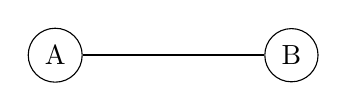
\begin{tikzpicture}[scale=1.5]

		\node[draw,circle] (A) at (0, 0) {A};
		\node[draw,circle] (B) at (2, 0) {B};

		\draw[thick] (A) -- (B);

	\end{tikzpicture}
\end{center}
\section{Arestas adjacentes(vizinhas)}
Arestas não paralelas podem ser consideradas adjacentes ou vizinhas caso sejam incidentes em um vértice comum
\dfnc{Arestas adjacentes}{Em um grafo $G = (V, E)$ é um par de arestas $e_1 = (u,v)$  $e_2 = (x, v) \mid e_1 \land  e_2 \in E$  }

\begin{center}
	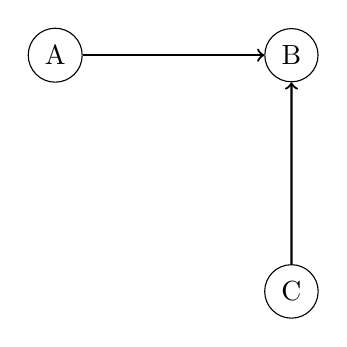
\begin{tikzpicture}[scale=1.5]

		\node[draw,circle] (A) at (0, 0) {A};
		\node[draw,circle] (B) at (2, 0) {B};
		\node[draw,circle] (C) at (2, -2) {C};

		\draw[->,thick] (A) -- (B);
		\draw[->,thick] (C) -- (B);

	\end{tikzpicture}
	\hspace{2cm}
	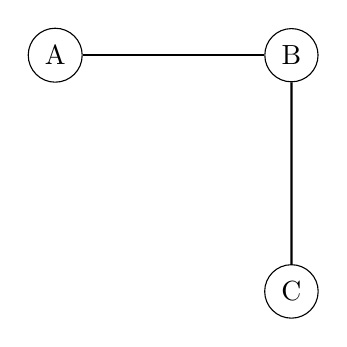
\begin{tikzpicture}[scale=1.5]

		\node[draw,circle] (A) at (0, 0) {A};
		\node[draw,circle] (B) at (2, 0) {B};
		\node[draw,circle] (C) at (2, -2) {C};

		\draw[thick] (A) -- (B);
		\draw[thick] (C) -- (B);

	\end{tikzpicture}
\end{center}

\section{Grafo Simples}
Um grafo simples é um grafo que não possui nem loops nem arestas parelelas

\begin{center}
	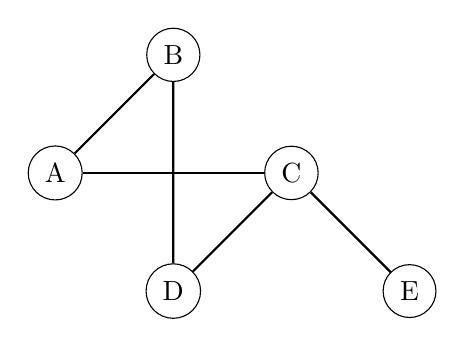
\begin{tikzpicture}[scale=1.5]

		\node[draw,circle] (A) at (0, 0) {A};
		\node[draw,circle] (B) at (1, 1) {B};
		\node[draw,circle] (C) at (2, 0) {C};
		\node[draw,circle] (D) at (1, -1) {D};
		\node[draw,circle] (E) at (3, -1) {E};

		\foreach \source/\dest in {A/B, A/C, B/D, C/D, C/E}
		\draw[thick] (\source) -- (\dest);

	\end{tikzpicture}
\end{center}

\subsection{Loop}

Um loop se trata de uma aresta associada a um par de vértices $(v_i, v_i)$
\dfnc{Loop}{
	Considerando um vértice $v_i$, um loop será definido por:

	\[
		\begin{aligned}
			E & = \{(v_i, v_j) \mid v_i, v_j \in V \mid  v_i = v_j \}
		\end{aligned}
	\]
}
\begin{center}
	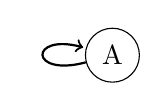
\begin{tikzpicture}[scale=1.5]

		\node[draw,circle] (A) at (0, 0) {A};

		\draw[->,thick] (A) edge[loop left] ();

	\end{tikzpicture}
\end{center}
\subsection{Arestas Parelelas}
Arestas Paralelas ocorrem quando existe mais de uma aresta associada ao mesmo par de vértices

\dfn{Arestas Paralelas}
{
	Para um Vértice $V_i $
	\[
		E = \{(v_i, v_j), (v_i, v_j), \dots \}
	\]

	Onde \(E\) é o conjunto de arestas tal que:

	\[
		E \subseteq V \times V
	\]

}

\begin{center}
	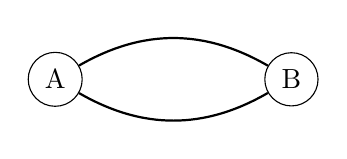
\begin{tikzpicture}[scale=1.5]

		\node[draw,circle] (A) at (0, 0) {A};
		\node[draw,circle] (B) at (2, 0) {B};

		\draw[-,thick] (A) to [bend left] (B);
		\draw[-,thick] (A) to [bend right] (B);

	\end{tikzpicture}
	\hspace{2cm}
	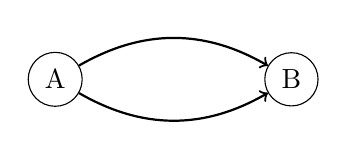
\begin{tikzpicture}[scale=1.5]

		\node[draw,circle] (A) at (0, 0) {A};
		\node[draw,circle] (B) at (2, 0) {B};

		\draw[->,thick] (A) to [bend left] (B);
		\draw[->,thick] (A) to [bend right] (B);

	\end{tikzpicture}
\end{center}
\nt{Importante ressaltar que as arestas para serem consideradas paralelas em um grafo direcionado, devem possuir o mesmo sentido/direção

	Exemplo de grafo sem arestas parelelas:
	\begin{center}
		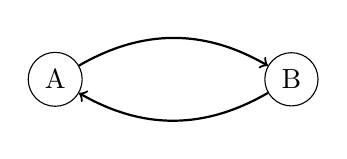
\begin{tikzpicture}[scale=1.5]

			\node[draw,circle] (A) at (0, 0) {A};
			\node[draw,circle] (B) at (2, 0) {B};

			\draw[->,thick] (A) to [bend left] (B);
			\draw[->,thick] (B) to [bend left] (A);

		\end{tikzpicture}
	\end{center}
}
\section{Graus}
\subsection{Grafo não direcionado}
Em um grafo não direcionado G =(V, E) , a quantidade de arestas em um vértice determina o seu grau $d(v)$

\begin{center}
	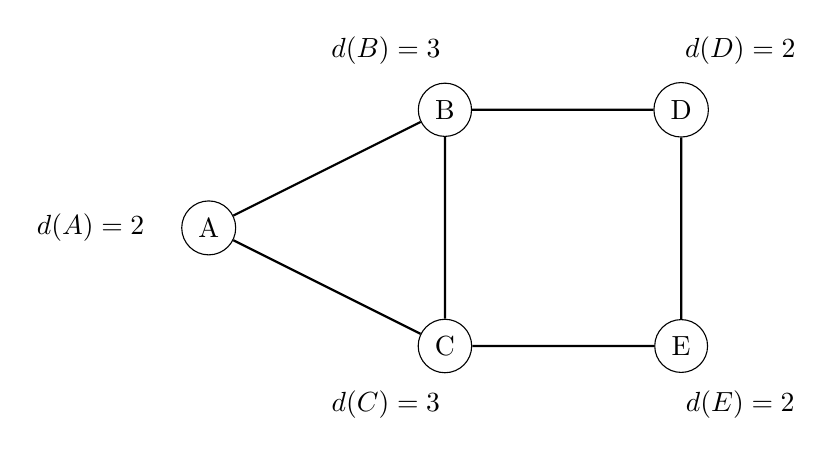
\begin{tikzpicture}[scale=1.5]

		\node[draw,circle] (A) at (0, 0) {A};
		\node[draw,circle] (B) at (2, 1) {B};
		\node[draw,circle] (C) at (2, -1) {C};
		\node[draw,circle] (D) at (4, 1) {D};
		\node[draw,circle] (E) at (4, -1) {E};

		\draw[thick] (A) -- (B);
		\draw[thick] (A) -- (C);
		\draw[thick] (B) -- (C);
		\draw[thick] (B) -- (D);
		\draw[thick] (C) -- (E);
		\draw[thick] (D) -- (E);


		\node at (-1, 0) {$d(A) = 2$};
		\node at (1.5, 1.5) {$d(B) = 3$};
		\node at (1.5, -1.5) {$d(C) = 3$};
		\node at (4.5, 1.5) {$d(D) = 2$};
		\node at (4.5, -1.5) {$d(E) = 2$};

	\end{tikzpicture}
\end{center}
\subsection{Grafo direcionado}
Em um grafo direcionado, existem dois tipos de graus, os de saída, que se referem as arestas que saem do determinado vértice $d^{+}(v)$, e de entrada, que se referem as arestas que chegam ao vértice $d^{-}(v)$

\begin{center}
	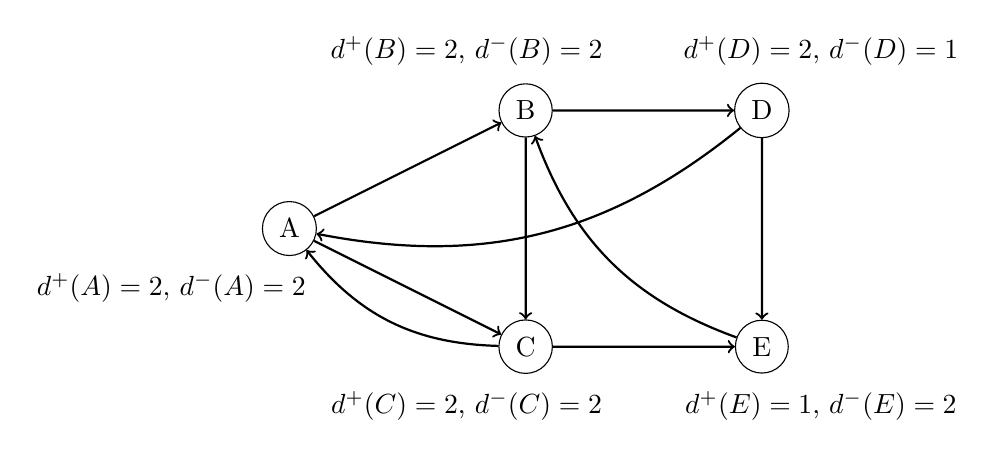
\begin{tikzpicture}[scale=1.5]

		\node[draw,circle] (A) at (0, 0) {A};
		\node[draw,circle] (B) at (2, 1) {B};
		\node[draw,circle] (C) at (2, -1) {C};
		\node[draw,circle] (D) at (4, 1) {D};
		\node[draw,circle] (E) at (4, -1) {E};

		\draw[->,thick] (A) -- (B);
		\draw[->,thick] (A) -- (C);
		\draw[->,thick] (B) -- (C);
		\draw[->,thick] (B) -- (D);
		\draw[->,thick] (C) -- (E);
		\draw[->,thick] (D) -- (E);

		\draw[->,thick, bend left=25] (C) to (A);
		\draw[->,thick, bend left=25] (E) to (B);
		\draw[->,thick, bend left=25] (D) to (A);

		\node at (-1, -0.5) {$d^{+}(A) = 2$, $d^{-}(A) = 2$};
		\node at (1.5, 1.5) {$d^{+}(B) = 2$, $d^{-}(B) = 2$};
		\node at (1.5, -1.5) {$d^{+}(C) = 2$, $d^{-}(C) = 2$};
		\node at (4.5, 1.5) {$d^{+}(D) = 2$, $d^{-}(D) = 1$};
		\node at (4.5, -1.5) {$d^{+}(E) = 1$, $d^{-}(E) = 2$};

	\end{tikzpicture}
\end{center}
\section{Fecho Transitivo Direto}
Para se falar de fecho transitivo direto, é a mesma coisa que falar da atingibilidade de um vértice, ou seja, quem é alcançavél a partir de um vértice $v$
\dfnc{Fecho Transitivo Direto}
{
	Dado um grafo $G = (V, E)$

	o seu fecho = v | vi, vj C E

}
\section{Caminho}
Caminho é uma sequência de vértices e arestas que começa e termina em um determinado vértice, que casso possua determinada características, possuirá um nome diferente, que são:
\subsection{Walk (Caminho)}
Um caminho é considerado "Walk", para qualquer caminho dentro de um grafo, sem nenhuma restrição além da definição básica de caminho.
\dfnc{Walk}
{
	Dado um caminho
	\[
		P = v_1, e_1, v_2, e_2,\dots,v_k
	\]
	onde:
	\[
		v_i \in V, \quad e_i \in E,
	\]
	conclui-se que:
	\[
		P = W
	\]

}
\subsection{Trail (Trilha)}
Um caminho é considerado "Trail", caso não possua repetição de arestas
\dfnc{Trail}
{
	Dado um caminho:
	\[
		P = v_1, e_1, v_2, e_2, \dots, v_k,
	\]
	onde:
	\[
		v_i \in V, \quad e_i \in E,
	\]
	se:
	\[
		e_i \neq e_j, \; \forall i \neq j,
	\]
	então:
	\[
		P = T.
	\]
}
\subsection{Path (Caminho simples)}
Um caminho é considerado Path, caso não possua repetição nem de vértices nem de arestas
\dfnc{Path}
{
	Dado um caminho:
	\[
		P = v_1, e_1, v_2, e_2, \dots, v_k,
	\]
	onde:
	\[
		v_i \in V, \quad e_i \in E,
	\]
	se:
	\[
		e_i \neq e_j, \; \forall i \neq j,
	\]
	e:
	\[
		v_i \neq v_j, \; \forall i \neq j,
	\]
	então:
	\[
		P = P_{simples}.
	\]
}
\section{Isomorfismo}
Dois grafos $G$ e $H$ são considerados isomorfos caso seja possível fazer uma relação de vértice para vértice e suas arestas entre todos os vértice de V, com as incidências também se mantendo


\begin{center}
	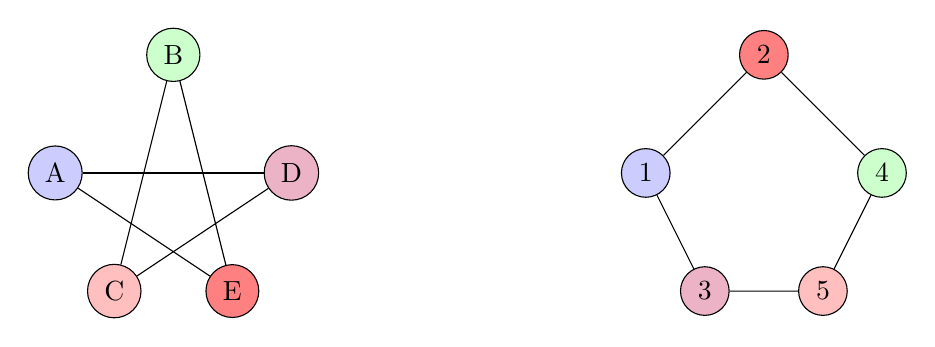
\begin{tikzpicture}[scale=1.5]

		\node[draw, circle, fill = blue!20] (A) at (0, 0) {A};
		\node[draw, circle, fill = green!20] (B) at (1, 1) {B};
		\node[draw, circle, fill = pink] (C) at (0.5, -1) {C};
		\node[draw, circle, fill = purple!30] (D) at (2, 0) {D};
		\node[draw, circle, fill = red!50] (E) at (1.5, -1) {E};

		\draw (A) -- (D);
		\draw (D) -- (C);
		\draw (C) -- (B);
		\draw (B) -- (E);
		\draw (E) -- (A);


		\node[draw, circle, fill = blue!20] (A2) at (5, 0) {1};
		\node[draw, circle, fill = red!50] (B2) at (6, 1) {2};
		\node[draw, circle, fill = purple!30] (C2) at (5.5, -1) {3};
		\node[draw, circle, fill = green!20] (D2) at (7, 0) {4};
		\node[draw, circle, fill = pink] (E2) at (6.5, -1) {5};

		\draw (A2) -- (B2);
		\draw (B2) -- (D2);
		\draw (C2) -- (E2);
		\draw (E2) -- (D2);
		\draw (A2) -- (C2);



	\end{tikzpicture}
\end{center}

\dfnc{Isomorfismo}
{
	Dado dois grafos
	\[
		G = (V, E) \text{ e } H = (V, E)
	\]
	que possuem:
	\[
		\text{Seq}_G = (d(u_1), d(u_2), \dots, d(u_n))
	\]
	\[
		\text{Seq}_H = (d(u_1), d(u_2), \dots, d(u_n))
	\]

	com as seguintes propriedades:

	\[
		|V_G| = |V_H|
	\]
	\[
		|E_G| = |E_H|
	\]
	\[
		\text{Seq}_G = \text{Seq}_H
	\]
	\[
		f: V_G \to V_H
	\]
	tal que, para quaisquer vértices \( u, v \in V_G \), temos:
	\[
		\{u, v\} \in E_G \iff \{f(u), f(v)\} \in E_H.
	\]
	apesar de não ser o suficiente para garantir, conclui-se que existe a possibilidade de:
	\[
		G \cong H
	\]

}
\nt{Essa definição apresenta propriedades necessárias, mas não suficientes, para garantir o isomorfismo. Mesmo que a correspondência dos vértices, arestas e graus seja necessária, não é suficiente para concluir o isomorfismo sem a condição de preservação de adjacência(relação entre arestas).}

\section{Grafo Completo}
Um grafo completo é um grafo que possui em seu conjunto de arestas E todas arestas possíveis do grafo.
\begin{center}
	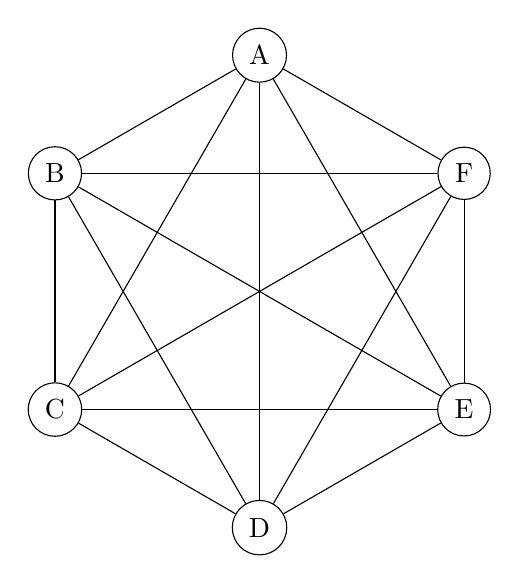
\begin{tikzpicture}[scale=3]

		\node[draw, circle] (A) at (90:1) {A};
		\node[draw, circle] (B) at (150:1) {B};
		\node[draw, circle] (C) at (210:1) {C};
		\node[draw, circle] (D) at (270:1) {D};
		\node[draw, circle] (E) at (330:1) {E};
		\node[draw, circle] (F) at (30:1) {F};

		\draw (A) -- (B);
		\draw (A) -- (C);
		\draw (A) -- (D);
		\draw (A) -- (E);
		\draw (A) -- (F);
		\draw (B) -- (C);
		\draw (B) -- (D);
		\draw (B) -- (E);
		\draw (B) -- (F);
		\draw (C) -- (D);
		\draw (C) -- (E);
		\draw (C) -- (F);
		\draw (D) -- (E);
		\draw (D) -- (F);
		\draw (E) -- (F);

	\end{tikzpicture}
\end{center}
\dfnc{Grafo Completo}
{
	Dado um grafo
	\[
		G = (V,E)
	\]
	onde:
	\[
		\mid E \mid = \frac{n \cdot (n - 1)}{2}
	\]
	\[
		\forall \, v \in V, \quad d(v) = n - 1
	\]
	Conclui-se que:
	\[
		G = K_n
	\]
}
\section{Grafo Complementar}
Um grafo complementar de um Grafo $G = (V,E)$ é um grafo $G' =  (V,E')$ em que suas arestas correpondem a todas arestas faltantes em G para se ter um grafo completo.
\begin{center}
	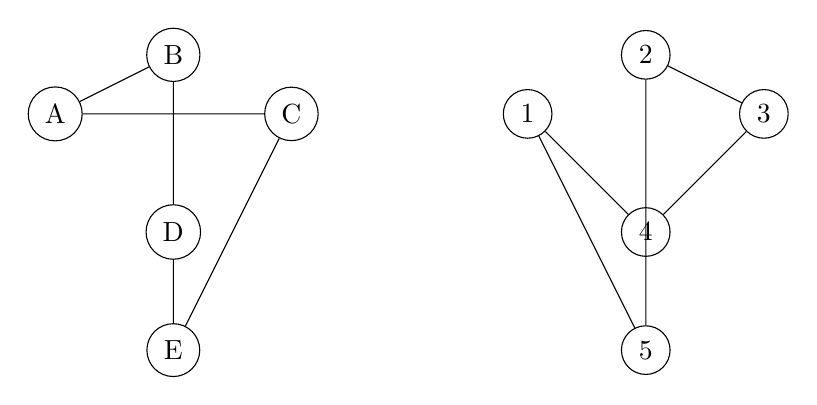
\begin{tikzpicture}[scale=1.5]

		\node[draw, circle] (A) at (0, 1) {A};
		\node[draw, circle] (B) at (1, 1.5) {B};
		\node[draw, circle] (C) at (2, 1) {C};
		\node[draw, circle] (D) at (1, 0) {D};
		\node[draw, circle] (E) at (1, -1) {E};

		\draw (A) -- (B);
		\draw (A) -- (C);
		\draw (B) -- (D);
		\draw (C) -- (E);
		\draw (D) -- (E);

		\node[draw, circle] (A2) at (4, 1) {1};
		\node[draw, circle] (B2) at (5, 1.5) {2};
		\node[draw, circle] (C2) at (6, 1) {3};
		\node[draw, circle] (D2) at (5, 0) {4};
		\node[draw, circle] (E2) at (5, -1) {5};

		\draw (A2) -- (D2);
		\draw (A2) -- (E2);
		\draw (B2) -- (C2);
		\draw (B2) -- (E2);
		\draw (C2) -- (D2);

	\end{tikzpicture}
\end{center}
\dfnc{Grafo Complementar}
{
	Dado dois grafos
	\[
		G = (V, E) \text{ e } G' = (V, E')
	\]
	onde:
	\[
		E \cap E' = \emptyset
	\]
	\[
		|E| + |E'| = \frac{n \cdot (n - 1)}{2}
	\]
	conclui-se que:
	\[
		E' = \overline{E}
	\]





}
\section{Subgrafo}
 {
  Dizemos que um Grafo é subgrafo de outro grafo, caso todos elementos(vértices e arestas) do subgrafo façam parte do outro Grafo


  \begin{center}
	  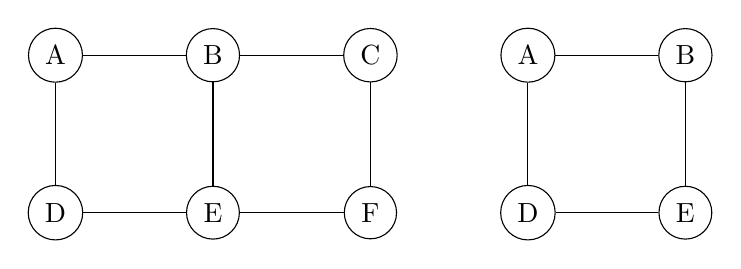
\begin{tikzpicture}
		  \node[circle, draw] (A) at (0, 2) {A};
		  \node[circle, draw] (B) at (2, 2) {B};
		  \node[circle, draw] (C) at (4, 2) {C};
		  \node[circle, draw] (D) at (0, 0) {D};
		  \node[circle, draw] (E) at (2, 0) {E};
		  \node[circle, draw] (F) at (4, 0) {F};

		  \draw (A) -- (B);
		  \draw (B) -- (C);
		  \draw (A) -- (D);
		  \draw (B) -- (E);
		  \draw (C) -- (F);
		  \draw (D) -- (E);
		  \draw (E) -- (F);

		  \node[circle, draw] (A1) at (6, 2) {A};
		  \node[circle, draw] (B2) at (8, 2) {B};
		  \node[circle, draw] (D3) at (6, 0) {D};
		  \node[circle, draw] (E4) at (8, 0) {E};

		  \draw (A1) -- (B2);
		  \draw (A1) -- (D3);
		  \draw (B2) -- (E4);
		  \draw (D3) -- (E4);
	  \end{tikzpicture}
  \end{center}

  \dfnc{Subgrafo}{
	  Dado dois grafos
	  \[
		  G = (V,E) \text{ e } H = (V,E)
	  \]
	  onde:
	  \[
		  V_H \subseteq V_G
	  \]
	  \[
		  E_H \subseteq E_G
	  \]
	  ou:
	  \[
		  \forall e \in E_H, \, e \in E_G
	  \]
	  \[
		  \forall v \in V_H, \, v \in V_G
	  \]

	  Conclui-se que:
	  \[
		  H \subseteq G
	  \]

  }
 }
\section{Ciclos}
Um grafo possui ciclos caso caso possua um caminho que possui o mesmo vértice de início e fim
Por exemplo o caminho: $P = A, AC, C, CD, D, DB, B, BA, A$
\begin{center}
	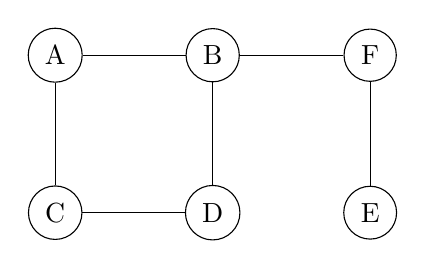
\begin{tikzpicture}
		\node[circle, draw] (A) at (0, 2) {A};
		\node[circle, draw] (B) at (2, 2) {B};
		\node[circle, draw] (C) at (0, 0) {C};
		\node[circle, draw] (D) at (2, 0) {D};
		\node[circle, draw] (E) at (4, 0) {E};
		\node[circle, draw] (F) at (4, 2) {F};

		\draw (A) -- (B);
		\draw (D) -- (C);
		\draw (A) -- (C);
		\draw (B) -- (D);
		\draw (B) -- (F);
		\draw (F) -- (E);

	\end{tikzpicture}
\end{center}
\dfnc{Ciclo}
{
	Dado um grafo
	\[
		G = (V, E)
	\]
	onde:
	\[
		P = v_1, e_1, v_2, e_2, v_3, e_3,\dots,v_k, e_k, v_1
	\]
	\[
		V' = \{v_2, v_3, \dots, v_k\} \text{	(todos vértices menos o $v_1$)}
	\]
	\[
		v_i \neq v_j, \; \forall v_i, v_j \in V', \; i \neq j
	\]
	\[
		e_i \neq e_j, \; \forall e_i, e_j \in E, \; i \neq j
	\]
	então:
	\[
		P = C
	\]


}
\section{Grafo Ciclo}
Um grafo Ciclo é um grafo que possui um caminho ciclo com todos seus vértices, ou seja, ele inteiro é um ciclo.

\begin{center}
	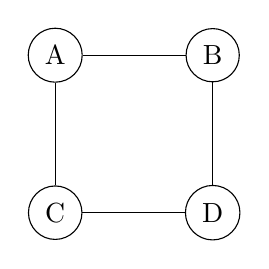
\begin{tikzpicture}
		\node[circle, draw] (A) at (0, 2) {A};
		\node[circle, draw] (B) at (2, 2) {B};
		\node[circle, draw] (C) at (0, 0) {C};
		\node[circle, draw] (D) at (2, 0) {D};

		\draw (A) -- (B);
		\draw (D) -- (C);
		\draw (A) -- (C);
		\draw (B) -- (D);

	\end{tikzpicture}
\end{center}
\dfnc{Grafo Ciclo}
{
Dado um grafo
\[
	G = (V,E)
\]
onde:
\[
	\forall v \in V, \;
\]
\[
	\mathcal{P}_{\text{max}}(v) = \underset{\mathcal{P} \in \; \mathcal{P}(v)}{\operatorname{arg\,max}} \, |E(\mathcal{P})| \; \land \; \mathcal{P}_{\text{max}}(v) = C
\]
então:
\[
	\mathcal{P}_{\text{max}}(v) = C_n
\]

}

\section{Termos}
\chapter{Algortimos}
\section{Busca em profundidade(DFS)}
A busca em profundidade
\chapter{}
\section{Random Examples}
\dfn{Limit of Sequence in $\bs{\bbR}$}{Let $\{s_n\}$ be a sequence in $\bbR$. We say $$\lim_{n\to\infty}s_n=s$$ where $s\in\bbR$ if $\forall$ real numbers $\eps>0$ $\exists$ natural number $N$ such that for $n>N$ $$s-\eps<s_n<s+\eps\text{ i.e. }|s-s_n|<\eps$$}
\qs{}{Is the set ${x-}$axis${\setminus\{\text{Origin}\}}$ a closed set}
\sol We have to take its complement and check whether that set is a open set i.e. if it is a union of open balls
\nt{We will do topology in Normed Linear Space  (Mainly $\bbR^n$ and occasionally $\bbC^n$)using the language of Metric Space}
\clm{Topology}{}{Topology is cool}
\ex{Open Set and Close Set}{
	\begin{tabular}{rl}
		Open Set:   & $\bullet$ $\phi$                                              \\
		            & $\bullet$ $\bigcup\limits_{x\in X}B_r(x)$ (Any $r>0$ will do) \\[3mm]
		            & $\bullet$ $B_r(x)$ is open                                    \\
		Closed Set: & $\bullet$ $X,\ \phi$                                          \\
		            & $\bullet$ $\overline{B_r(x)}$                                 \\
		            & $x-$axis $\cup$ $y-$axis
	\end{tabular}}
\thm{}{If $x\in$ open set $V$ then $\exists$ $\delta>0$ such that $B_{\delta}(x)\subset V$}
\begin{myproof}By openness of $V$, $x\in B_r(u)\subset V$
	\begin{center}
		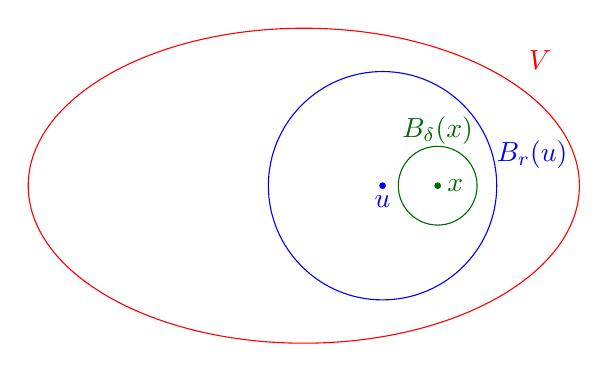
\begin{tikzpicture}
			\draw[red] (0,0) circle [x radius=3.5cm, y radius=2cm] ;
			\draw (3,1.6) node[red]{$V$};
			\draw [blue] (1,0) circle (1.45cm) ;
			\filldraw[blue] (1,0) circle (1pt) node[anchor=north]{$u$};
			\draw (2.9,0.4) node[blue]{$B_r(u)$};
			\draw [green!40!black] (1.7,0) circle (0.5cm) node [yshift=0.7cm]{$B_{\delta}(x)$} ;
			\filldraw[green!40!black] (1.7,0) circle (1pt) node[anchor=west]{$x$};
		\end{tikzpicture}
	\end{center}

	Given $x\in B_r(u)\subset V$, we want $\delta>0$ such that $x\in B_{\delta} (x)\subset B_r(u)\subset V$. Let $d=d(u,x)$. Choose $\delta $ such that $d+\delta<r$ (e.g. $\delta<\frac{r-d}{2}$)

	If $y\in B_{\delta}(x)$ we will be done by showing that $d(u,y)<r$ but $$d(u,y)\leq d(u,x)+d(x,y)<d+\delta<r$$
\end{myproof}

\cor{}{By the result of the proof, we can then show...}
\mlenma{}{Suppose $\vec{v_1}, \dots, \vec{v_n} \in \RR[n]$ is subspace of $\RR^n$.}
\mprop{}{$1 + 1 = 2$.}

\section{Random}
\dfn{Normed Linear Space and Norm $\boldsymbol{\|\cdot\|}$}{Let $V$ be a vector space over $\bbR$ (or $\bbC$). A norm on $V$ is function $\|\cdot\|\ V\to \bbR_{\geq 0}$ satisfying \begin{enumerate}[label=\bfseries\tiny\protect\circled{\small\arabic*}]
		\item \label{n:1}$\|x\|=0 \iff x=0$ $\forall$ $x\in V$
		\item \label{n:2}	$\|\lambda x\|=|\lambda|\|x\|$ $\forall$ $\lambda\in\bbR$(or $\bbC$), $x\in V$
		\item \label{n:3} $\|x+y\| \leq \|x\|+\|y\|$ $\forall$ $x,y\in V$ (Triangle Inequality/Subadditivity)
	\end{enumerate}And $V$ is called a normed linear space.

	$\bullet $ Same definition works with $V$ a vector space over $\bbC$ (again $\|\cdot\|\to\bbR_{\geq 0}$) where \ref{n:2} becomes $\|\lambda x\|=|\lambda|\|x\|$ $\forall$ $\lambda\in\bbC$, $x\in V$, where for $\lambda=a+ib$, $|\lambda|=\sqrt{a^2+b^2}$ }


\ex{$\bs{p-}$Norm}{\label{pnorm}$V={\bbR}^m$, $p\in\bbR_{\geq 0}$. Define for $x=(x_1,x_2,\cdots,x_m)\in\bbR^m$ $$\|x\|_p=\Big(|x_1|^p+|x_2|^p+\cdots+|x_m|^p\Big)^{\frac1p}$$(In school $p=2$)}
\textbf{Special Case $\bs{p=1}$}: $\|x\|_1=|x_1|+|x_2|+\cdots+|x_m|$ is clearly a norm by usual triangle inequality. \par
\textbf{Special Case $\bs{p\to\infty\ (\bbR^m$ with $\|\cdot\|_{\infty})}$}: $\|x\|_{\infty}=\max\{|x_1|,|x_2|,\cdots,|x_m|\}$\\
For $m=1$ these $p-$norms are nothing but $|x|$.
Now exercise
\qs{}{\label{exs1}Prove that triangle inequality is true if $p\geq 1$ for $p-$norms. (What goes wrong for $p<1$ ?)}
\sol{\textbf{For Property \ref{n:3} for norm-2}	\subsubsection*{\textbf{When field is $\bbR:$}} We have to show\begin{align*}
		         & \sum_i(x_i+y_i)^2\leq \left(\sqrt{\sum_ix_i^2} +\sqrt{\sum_iy_i^2}\right)^2                                       \\
		\implies & \sum_i (x_i^2+2x_iy_i+y_i^2)\leq \sum_ix_i^2+2\sqrt{\left[\sum_ix_i^2\right]\left[\sum_iy_i^2\right]}+\sum_iy_i^2 \\
		\implies & \left[\sum_ix_iy_i\right]^2\leq \left[\sum_ix_i^2\right]\left[\sum_iy_i^2\right]
	\end{align*}So in other words prove $\langle x,y\rangle^2 \leq \langle x,x\rangle\langle y,y\rangle$ where
	$$\langle x,y\rangle =\sum\limits_i x_iy_i$$

	\begin{note}
		\begin{itemize}
			\item $\|x\|^2=\langle x,x\rangle$
			\item $\langle x,y\rangle=\langle y,x\rangle$
			\item $\langle \cdot,\cdot\rangle$ is $\bbR-$linear in each slot i.e. \begin{align*}
				      \langle rx+x',y\rangle=r\langle x,y\rangle+\langle x',y\rangle	\text{ and similarly for second slot}
			      \end{align*}Here in $\langle x,y\rangle$ $x$ is in first slot and $y$ is in second slot.
		\end{itemize}
	\end{note}Now the statement is just the Cauchy-Schwartz Inequality. For proof $$\langle x,y\rangle^2\leq \langle x,x\rangle\langle y,y\rangle $$ expand everything of $\langle x-\lambda y,x-\lambda y\rangle$ which is going to give a quadratic equation in variable $\lambda $ \begin{align*}
		\langle x-\lambda y,x-\lambda y\rangle & =\langle x,x-\lambda y\rangle-\lambda\langle y,x-\lambda y\rangle                                       \\
		                                       & =\langle x ,x\rangle -\lambda\langle x,y\rangle -\lambda\langle y,x\rangle +\lambda^2\langle y,y\rangle \\
		                                       & =\langle x,x\rangle -2\lambda\langle x,y\rangle+\lambda^2\langle y,y\rangle
	\end{align*}Now unless $x=\lambda y$ we have $\langle x-\lambda y,x-\lambda y\rangle>0$ Hence the quadratic equation has no root therefore the discriminant is greater than zero.

	\subsubsection*{\textbf{When field is $\bbC:$}}Modify the definition by $$\langle x,y\rangle=\sum_i\overline{x_i}y_i$$Then we still have $\langle x,x\rangle\geq 0$}

\section{Algorithms}
\begin{algorithm}[H]
	\KwIn{This is some input}
	\KwOut{This is some output}
	\SetAlgoLined
	\SetNoFillComment
	\tcc{This is a comment}
	\vspace{3mm}
	some code here\;
	$x \leftarrow 0$\;
	$y \leftarrow 0$\;
	\uIf{$ x > 5$} {
		x is greater than 5 \tcp*{This is also a comment}
	}
	\Else {
		x is less than or equal to 5\;
	}
	\ForEach{y in 0..5} {
		$y \leftarrow y + 1$\;
	}
	\For{$y$ in $0..5$} {
		$y \leftarrow y - 1$\;
	}
	\While{$x > 5$} {
		$x \leftarrow x - 1$\;
	}
	\Return Return something here\;
	\caption{what}
\end{algorithm}

\end{document}
